\documentclass[11pt,letterpaper]{article}

\input{../../../../.config/latex/preamble_v1.tex}
\lightmode

% Disable algorithm numbering
\renewcommand{\thealgocf}{}

\begin{document}

\section*{CS 124 Homework 2: Spring 2022}
\textbf{Your name:} Lev Kruglyak 

\textbf{Collaborators:} Swati Goel, Katrina Brown, Sahil Kuchlous

\textbf{No. of late days used on previous psets: } 0\\
\textbf{No. of late days used after including this pset: } 2

Homework is due Wednesday at midnight ET. You are allowed up to {\bf twelve} 
(college)/{\bf forty} (extension school) late days through the semester, but the number of late days you take on each assignme\ nt must be a nonnegative integer at most {\bf two} (college)/{\bf four} (extension school).

Try to make your answers as clear and concise as possible; style may count in your grades. Assignments must be submitted in pdf format on Gradescope. If you do assignments by hand, you will need to scan in your results to
turn them in.

You can collaborate with other students that are currently enrolled in this course in brainstorming and thinking through approaches to solutions but you should write the solutions on your own: you must wait one hour after any collaboration or use of notes from collaboration before any writing in your own solutions that you will submit.

For all homework problems where you are asked to give an algorithm, you must prove the correctness of your algorithm and establish the best upper bound that you can give for the running time. Generally better running times will get better credit; generally exponential time algorithms (unless specifically asked for) will receive no or little credit. You should always write a clear informal description of your algorithm in English. You may also write pseudocode if you feel your informal explanation requires more precision and detail, but keep in mind pseudocode does NOT substitute for an explanation. Answers that consist
solely of pseudocode will receive little or not credit. Again, try to make your 
answers clear and concise.

\pagebreak
\begin{problem}\noindent
    \begin{enumerate}[(a)]
        \item {\bf (7 points)} We saw in lecture that we can find a topological sort of a directed acyclic graph by running DFS and ordering according to the postorder time (that is, we add a vertex to the sorted list \emph{after} we visit its out- neighbors).  Suppose we try to build a topological sort by ordering in increasing order according to the preorder, and not the postorder, time.  Give a counterexample to show this doesn't work, and explain why it's a counterexample.  
        \item {\bf (7 points)} Same as above, but we try to sort by decreasing preorder time.
        \end{enumerate}
\end{problem}

\begin{solution}
    Consider the following directed acylcic graph:
    \begin{center}
        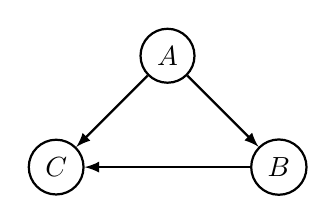
\begin{tikzpicture}[node distance={20mm}, thick, main/.style = {draw, circle}]
            \node[main] (1) {$A$}; 
            \node[main] (2) [below right of=1] {$B$}; 
            \node[main] (3) [below left of=1] {$C$}; 

            \draw[-latex] (1) -- (2); 
            \draw[-latex] (1) -- (3); 
            \draw[-latex] (2) -- (3);
        \end{tikzpicture}
    \end{center}
    Running a DFS on this graph gives the following preorder and postorder times:
    \begin{center}
        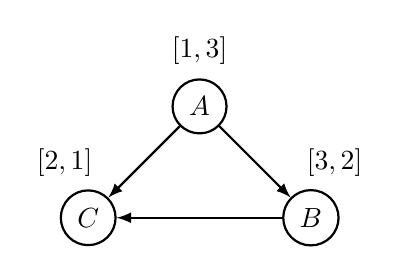
\begin{tikzpicture}[node distance={20mm}, thick, main/.style = {draw, circle}]
            \node[main] (1) {$A$}; 
            \node[main] (2) [below right of=1] {$B$}; 
            \node[main] (3) [below left of=1] {$C$}; 

            \draw[-latex] (1) -- (2); 
            \draw[-latex] (1) -- (3); 
            \draw[-latex] (2) -- (3);

            \node at (1) [left = 0mm, above=4mm] {$[1,3]$};
            \node at (2) [right = 3mm, above=4mm] {$[3,2]$};
            \node at (3) [left = 3mm, above=4mm] {$[2,1]$};
        \end{tikzpicture}
    \end{center}
    If we try building a topological sort by sorting by the usual postorder time, we get:
    \begin{center}
        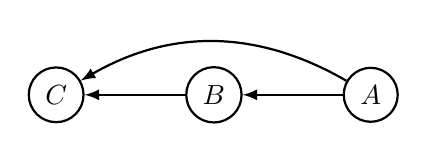
\begin{tikzpicture}[node distance={20mm}, thick, main/.style = {draw, circle}]
            \node[main] (1) [right=0mm] {$C$};
            \node[main] (2) [right=20mm] {$B$};
            \node[main] (3) [right=40mm] {$A$};

            \draw[-latex] (2) to (1);
            \draw[-latex] (3) to [out=150,in=30] (1);
            \draw[-latex] (3) to (2);
        \end{tikzpicture}
    \end{center}
    This is clearly a valid topological sort because all of the directed edges point in the same direction, i.e. there are back edges. If we instead sort by the increasing preorder time, we get:
    \begin{center}
        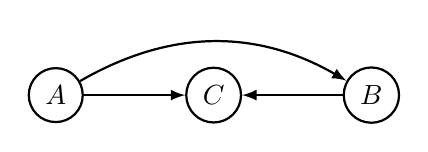
\begin{tikzpicture}[node distance={20mm}, thick, main/.style = {draw, circle}]
            \node[main] (1) [right=0mm] {$A$};
            \node[main] (2) [right=20mm] {$C$};
            \node[main] (3) [right=40mm] {$B$};

            \draw[-latex] (1) to (2);
            \draw[-latex] (1) to [out=30,in=150] (3);
            \draw[-latex] (3) to (2);
        \end{tikzpicture}
    \end{center}
    This is not a valid topological sort because all the directed edges aren't pointing in the same direction. The same thing happens if we sort by decreasing preorder time.
    \begin{center}
        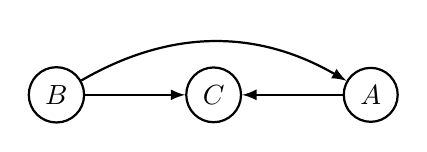
\begin{tikzpicture}[node distance={20mm}, thick, main/.style = {draw, circle}]
            \node[main] (3) [right=40mm] {$A$};
            \node[main] (2) [right=20mm] {$C$};
            \node[main] (1) [right=0mm] {$B$};

            \draw[-latex] (1) to (2);
            \draw[-latex] (1) to [out=30,in=150] (3);
            \draw[-latex] (3) to (2);
        \end{tikzpicture}
    \end{center}
\end{solution}

\pagebreak
\begin{problem}
    {\bf (20 points)} News from Cambridge: every night, snow falls and covers all the sidewalks.  Every morning, the city's lone snow shoveler, Pat, is tasked with clearing all the sidewalks of snow. Proper snow-shoveling technique requires that sidewalks on opposite sides of the same street be shoveled in opposite directions.  (Every street has sidewalks on both sides.) Give an algorithm to find a snow-shoveling path for Pat that doesn't require any more walking than necessary---at most once per sidewalk.  (If you have to assume anything about the layout of the city of Cambridge, make it clear!) (Your algorithm should work for any city, not just the Cambridge in which Harvard is.)
\end{problem}

\begin{solution}
    This problem can be represented as a graph by letting points represent street intersections and edges represent streets. Since the sidewalks must go both ways (assuming there are no one-way sidewalks), this is an undirected graph. To keep this a graph and not a multi-graph, we must further assume that there can only be a single street connecting two intersections. This isn't super important since we can always add intersections to eliminate duplicate edges. Lastly we assume that the graph is connected, i.e. every two points in the city can be reached by walking on sidewalks. Otherwise Pat would have to venture into the wilderness to access a neighboring connected component, which may be outside of the job description. We can now finally present the algorithm:

    \RestyleAlgo{ruled}
    \begin{algorithm}
    \caption{Efficient Snow Shovelling}
    \DontPrintSemicolon
    \SetKwFunction{shovel}{shovel}
    \SetKwProg{myalg}{procedure}{}{}

    \myalg{\shovel{$u,v\in V$}} {
        assuming Pat is at $u$, shovel the sidewalk from $u$ to $v$.\;
        Pat should now be at $v$.
    }\;

    \SetKwFunction{recursiveShovel}{recursive\_shovel}
    
    $\forall (i,j)\in E, e[i,j]\leftarrow 0$ \Comment*[r]{start all edges as not shovelled}
    \myalg{\recursiveShovel{$G(V,E), s\in V$}}{
        \For(){$(s,v)\in E$}{
            \If(){$e[s,v] = 0$ or $e[v,s]=0$}{
                $e[s,v], e[v,s]\leftarrow 1$\Comment*[r]{mark edge as shovelled} 
                \shovel{$s,v$}\Comment*[r]{point A}
                \recursiveShovel{$G, v$}\;
                \shovel{$v,s$}\Comment*[r]{point B}
            }
        }
    }
    \end{algorithm}

    First we'll prove that this algorithm produces a well-defined motion of Pat. (i.e. \shovel{$u,v$} is only called when Pat is at $u$) More formally, we can show that \recursiveShovel{$G,s$} does not move Pat after completing, i.e. when called, Pat starts at $s$ and when the function finishes, Pat is still at $s$. For the base case when \recursiveShovel{$G,s$} returns immediately because all of its adjacent edges have already been explored, Pat does not move at all by assumption. Next, for the inductive step and assuming that \recursiveShovel{$G,s$} works for smaller subtrees, note that the block of code from point A to point B does not actually move Pat at all; \shovel{$s,v$} moves Pat to $v$, by the inductive step \recursiveShovel{$G,v$} keeps Pat at $v$, and \shovel{$v,s$} moves Pat back to $s$. This completes the proof of well-definedness.   

    Finally, we claim that running \recursiveShovel{$G,s$} on any $s\in V$ will call \shovel{$u,v$} and \shovel{$v,u$} exactly once for each edge $(u,v)\in E$; this is exactly the problem of shovelling snow. First of all note that this algorithm performs a DFS (depth first search) of the graph, so by an elementary property of DFS, the \shovel{$s,v$} command at point A is called only once for every edge in the graph.Since it comes paired with the reverse shovel command at point B, it follows that \shovel{$u,v$} and \shovel{$v,u$} are called exactly once for every edge $(u,v)\in E$, as requested. 
    
\end{solution}

\pagebreak
\begin{problem}
    {\bf (0 points, optional)} This exercise is based on the 2SAT problem.  The input to 2SAT is a logical expression of a specific form:  it is the conjunction (AND) of a set of clauses, where each clause is the disjunction (OR) of two literals.  (A literal is either a Boolean variable or the negation of a Boolean variable.)  For example, the following expression is an instance of 2SAT:
    
    \[ (x_1 \, \vee \, \overline{x_2}) \wedge (\overline{x_1} \, \vee \, \overline{x_3}) \wedge (x_1 \, \vee \, x_2) \wedge (x_4 \, \vee \, \overline{x_3}) \wedge (x_4 \, \vee \, \overline{x_1}).\]

    A solution to an instance of a 2SAT formula is an assignment of the variables to the values T (true) and F (false) so that all the clauses are satisfied-- that is, there is at least one true literal in each clause. For example, the assignment $x_1 = T, x_2 = F, x_3 = F, x_4 = T$ satisfies the 2SAT formula above.\\\hspace*{\fill}

    Derive an algorithm that either finds a solution to a 2SAT formula, or returns that no solution exists. Carefully give a complete description of the entire algorithm and the running time.  (Hint: Reduce to an appropriate problem.  It may help to consider the following directed graph, given a formula $I$ in 2SAT: the nodes of the graph are all the variables appearing in $I$, and their negations.  For each clause $(\alpha \, \vee \, \beta)$ in $I$, we add a directed edge from $\overline{\alpha}$ to $\beta$ and a second directed edge from $\overline{\beta}$ to $\alpha$.  How can this be interpreted?)
\end{problem}

\begin{solution}
    
\end{solution}

\pagebreak
\begin{problem}
    {\bf (15 points)} The {\em risk-free currency exchange problem} offers a risk-free way to make money.  Suppose we have currencies $c_1,\ldots,c_n$. (For example, $c_1$ might be dollars, $c_2$ rubles, $c_3$ yen, etc.)  For various pairs of distinct currencies $c_i$ and $c_j$ (but not necessarily every pair!) there is an exchange rate $r_{i,j}$ such that you can exchange one unit of $c_i$ for $r_{i,j}$ units of $c_j$.  (Note that even if there is an exchange rate $r_{i,j}$, so it is possible to turn currency $i$ into currency $j$ by an exchange, the reverse might not be true--- that is, there might not be an exchange rate $r_{j,i}$.)  Now if, because of exchange rate strangeness, $r_{i,j} \cdot r_{j,i} > 1$, then you can make money simply by trading units of currency $i$ into units of currency $j$ and back again.  (At least, if there are no exchange costs.) This almost never happens, but occasionally (because the updates for exchange rates do not happen quickly enough) for very short periods of time exchange traders can find a sequence of trades that can make risk-free money. That is, if there is a sequence of currencies $c_{i_1},c_{i_2},\ldots,c_{i_k}$ such that $r_{{i_1},{i_2}} \cdot r_{{i_2},{i_3}} \ldots \cdot r_{{i_{k-1}},{i_k}} \cdot r_{{i_k},{i_1}} > 1$, then trading one unit of $c_{i_1}$ into $c_{i_2}$ and trading that into $c_{i_3}$ and so on back to $c_{i_1}$ will yield a profit.  Design an efficient algorithm to detect if a risk-free currency exchange exists. (You need not actually find it.)
\end{problem}

\begin{solution}
    We'll represent this system of currencies as a weighed directed graph $G(V,E,w)$ with a vertex for each currency $c_i$, an edge for each known currency exchange between two currencies, and a weight function which takes a currency exchange edge $(c_i, c_j)$ to the corresponding value $r_{i,j}$. All of the weights are positive by assumption, so we may start to interpret them as some form of distance. Exchange rates are multiplicative, so rather than add distances we multiply them. The problem of finding a risk-free currency exchange then becomes the problem of finding a cycle of vertices $v_0\to v_1\to\cdots\to v_n\to v_0$ with $w(v_0, v_1)\cdots w(v_{n-1},v_n) \cdot w(v_n, v_0) > 1$.
    
    This is just a multiplicative variant of the problem to find negative weight cycles in a weighted directed graph and can thus be solved using a multiplicative version of Bellman-Ford algorithm: 

    \RestyleAlgo{ruled}
    \begin{algorithm}
    \caption{Modified Bellman Ford}
    \DontPrintSemicolon
    \SetKwFunction{mbellmanford}{ModifiedBellmanFord}
    \SetKwProg{myalg}{procedure}{}{}
    
    \myalg{\mbellmanford{$G(V,E,w), s\in V$}}{
        $\forall v\in V,\; d[v]\leftarrow \infty$ \Comment*[r]{set initial distance estimates to infinity}
        $s\in V$, $d[s]\leftarrow 1$ \Comment*[r]{weight is multiplicative, so start w/ one}
        \For(){$i$ from $1\to n-1$}{
            \For(){$(u,v)\in E$}{
                $d[u]\leftarrow \min\{d[u], d[v]\cdot w(u,v)\}$ \Comment*[r]{update distance estimate}
            }
        }
        \For(){$(u,v)\in R$}{
            \If(){$d[u] > d[v]\cdot w(u,v)$ \Comment*[r]{risk-free currency exchange detected}}{\Return{true}}
        }
        \Return{false}
    }
    \end{algorithm}
    
    So \mbellmanford{$G,s$} will return true if and only if there is a risk-free currency exchange reachable from $s$, this follows from the standard Bellman-Ford algorithm. Note that its complexity is the same as the regular Bellman-Ford algorithm, $O(|V|\cdot |E|)$. However picking a random point and running \mbellmanford{$G,s$} won't necessarily find all of the risk free currency exchanges, since not every risk free currency exchange loop is reachable from $s$. So prior to running \mbellmanford{$G,s$}, we reverse the graph, run DFS at every point and list the nodes which have no outgoing edges. This takes $O(|V|\cdot |E|)$ time, and it will generate a list $S$ of the root vertices for all the strongly connected components in the graph. If we run \mbellmanford{$G,s$} for every $s\in S$, we now have an accurate assesment of the risk free currency exchanges in the currency market.
\end{solution}

\pagebreak
\begin{problem}
    {\bf (20 points)} Suppose that you are given a directed graph $G=(V,E)$ along with weights on the edges (you can assume that they are all positive). You are also given a vertex $s$ and a tree $T$ connecting the graph $G$ that is claimed to be the tree of shortest paths from $s$ that you would get using Dijkstra's algorithm.  Can you check that $T$ is correct in linear time?
\end{problem} 

% push S, v;
% while (S is not empty) do
%    u := pop S;
%    if (not visited[u]) then
%       visited[u] := true;
%       for each unvisited neighbour w of u
%          push S, w;
%    end if
% end while

\begin{solution}
    Yes, here is a simple algorithm to do so. First, we populate a set of shortest distances to each node from $s$ according to $T$. This has time complexity $O(|E|)$. 
    \RestyleAlgo{ruled}
    \begin{algorithm}
        \caption{Populate distance}
        \DontPrintSemicolon
        $\forall v\in V,\;d[v]\leftarrow \infty$ \Comment*[r]{set initial distance estimates }
        \SetKwFunction{populateDistance}{populateDistance}
        \SetKwProg{myalg}{procedure}{}{}
        \myalg{\populateDistance{$\textrm{vertex } s_0$, $\textrm{distance }d_0$}}{
            $d[s_0]\leftarrow d_0$\;
            \For(){$(s_0,v)\in T$}{
                \If(sanity check to prevent infinite loop. Won't happen if $T$ is actually a tree.){$d[v]=\infty$}{
                    \populateDistance{$v$, $d_0+w(s_0,v)$}
                }
            }  
            }
    \end{algorithm}
    Next, we run a single iteration of Bellman-Ford and see if there are any updates at all to the distance list. If this distance set is indeed minimal, then there will be no updates.
    \RestyleAlgo{ruled}
    \begin{algorithm}
        \caption{Dijkstra Verification}
        \DontPrintSemicolon
        \populateDistance{$s$, $0$}\;
        \For(){$(u,v)\in E$ }{
            \If(){$d[v] > w(u,v) + d[u]$}{
                \Return{false}
            }
        }
        \Return{true}
    \end{algorithm}
    The above algorithm is $O(|E|+|E|)=O(|E|)$ which is linear.
    It works because the shortest distance list can be obtained from scratch using the full Bellman-Ford algorithm. However if running a single update of Bellman-Ford does nothing, running all $|V|-1$ updates will do nothing, meaning the distance list is already correct. So if the tree is wrong, then the algorithm will return false, since there will be an update in the Bellman-Ford iteration. If the tree is correct, the algorithm will return true, since there cannot be any updates in the Bellman-Ford iteration. Thus the algorithm works correctly in all cases.
\end{solution}

\pagebreak
\begin{problem}
    Patients who require a kidney transplant but do not have a compatible donor can enter a kidney exchange. In this exchange, patient-donor pairs $p_i-d_i$ may be able to donate to each other: there's an input function $c$ such that for each pair $(i,j)$ of patient-donor pairs, either $c(i,j) = 1$ and $d_i$ can donate a kidney to $p_j$, or $c(i,j) = 0$ and $d_i$ can't donate a kidney to $p_j$. As an example, suppose that we have patient-donor pairs: $$p_1-d_1, p_2-d_2, p_3-d_3, p_4-d_4, p_5-d_5,$$  that $c(3,2) = c(3,1) = c(2,1) = c(1,3) = 1$, and that for all other inputs $c$ is 0. That is, in this example, $d_3$ can donate to $p_2$ or $p_1$, $d_2$ can donate to $p_1$, and $d_1$ can then donate to $p_3$ in the original $p_3-d_3$ pair. Then a set of these donations can simultaneously occur: all those donations except $d_3 \to p_1$ could happen simultaneously, with $p_4- d_4$ and $p_5-d_5$ not participating. For every donor that donates a kidney, their respective patient must also receive a kidney, so if instead $c(1,3) = 0$, no donations could occur: $d_3$ will refuse to donate a kidney to $p_2$ because $p_3$ won't get a kidney.
    \begin{enumerate}[(a)]
        \item {\bf (5 points)} Give an algorithm that determines whether or not a set of donations can occur. 
        \item {\bf (20 points)} Suppose that no set of donations can occur in the previous part, but we add of an altruistic donor, $d_0$. This altruistic donor is not bound to a patient, and is unconditionally willing to donate a kidney.  Additionally, for each donation from $d_i$ to $p_j$, consider that there is some value $v_{ij}$ associated with that donation. Give an algorithm that returns the highest value donation sequence. For partial credit, you can consider the cases where 1) every donation has the same value or 2) donations have possibly-distinct but only positive values. 
        \end{enumerate} 
\end{problem}

\begin{solution}
    Let's represent this problem as a directed graph, with vertices representing patient-donor pairs and a directed edge connecting pair $i$ to pair $j$ if and only if $c(i,j)=1$. 

    \textbf{(a)} Clearly a set of donations can occur if and only if there is a cycle in the graph because every node in the cycle will have exactly one edge going in and out of it. To detect edges in a graph, we can pick some starting point and attempt to perform a topological sort of the graph using a postorder ordering from a DFS (depth first search). Then if the resulting sort contains a back edge, there must be a cycle in the graph, and so a donation is possible. We repeat this for every patient donor pair in the graph to ensure that we have found all cycles.
    
    \textbf{(b)} Here we'll do the same thing, but now we also weigh edges with their donation value. Note that this graph is now a directed acyclic graph, since by assumption there is no donation sequence and so the graph contains no cycles. Also adding the single altruistic donor cannot add a cycle, since the donor is an extra vertex with only one outgoing edge. Now the problem of finding a valid donation sequence is the same as finding a path of highest weight in the graph. Note that such a path must necessarily start at $s_0$, the altruistic donor we added. Otherwise, we would need a cycle to satisfy the patient-donor requirement. So first let's run a topological sort starting at $s_0$. Then we can populate a list of distances to each vertex from $s_0$, remember the largest one, and then trace a longest path to it using the topological sort. All of these steps take linear time.
\end{solution}

\pagebreak
\begin{problem}
    Tony Stark has been thinking about how he can be more effective as Iron-Man and he's finally figured it out: two Iron-Men! He has two Iron-Man suits and he can control each remotely. Unfortunately, he's been having trouble getting the technology exactly right, so every time he makes a move in one suit, the other suit follows with a different move. Precisely, if Iron-Man 1 moves right, Iron-Man 2 moves up; if IM1 moves left, IM2 moves down; if IM1 moves up, IM2 moves left; and if IM1 moves down, then IM2 moves right. To slow him down, Thanos dropped one suit in Los Angeles and the other in Dallas. Tony needs your help getting both his suits back to Stark Industries in New York. 
 
    Because of COVID-related travel restrictions, the Iron-Men cannot leave the United States. For the sake of this problem, assume that the United States can be modelled as an $n$ by $n$ grid, as below (climate change has shaved off the East and West coasts). 
 
    \begin{center}
        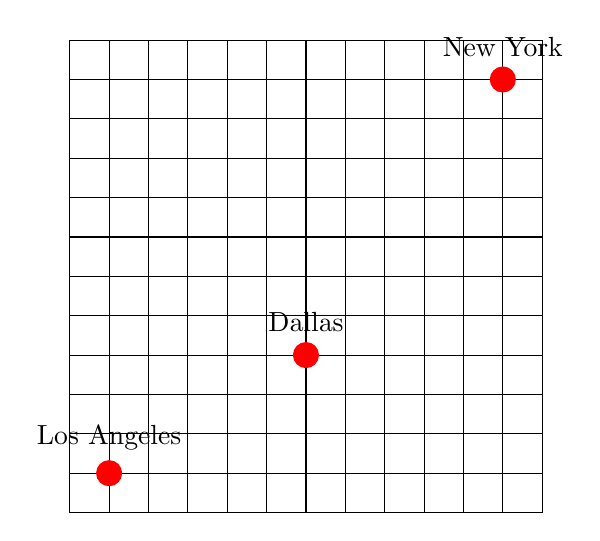
\begin{tikzpicture}
            \draw[step=.5cm] (-3, -3) grid (3, 3);
            \node[label={Los Angeles}, circle, fill=red, minimum size= 0.01cm] at (-2.5, -2.5) {};
            \node[label={Dallas}, circle, fill=red, minimum size= 0.01cm] at (0, -1) {};
            \node[label={New York}, circle, fill=red, minimum size= 0.01cm] at (2.5, 2.5) {};
        \end{tikzpicture}
    \end{center}

    If an Iron-Man tries to move off the grid or into an obstacle, it merely stays in place. Additionally, each step has a cost that depends on the robot's location. For example, moving left from (0, 1) might cost 1 fuel but moving left from (10, 15) might require jumping over someone's backyard pool and thus might cost 3 fuels.  Once a robot reaches Stark Industries, it powers down and costs 0 fuels even as its counterpart continues to move. You are given the positions of Los Angeles ($x_\ell, y_\ell$), Dallas ($x_d, y_d$), and New York ($x_{ny}, y_{ny}$), the positions of all obstacles $(x_{o_i}, y_{o_i})$, and the cost of every possible move from every possible location.

    \begin{enumerate}[(a)]
        \item {\bf (10 points)} Give and explain an asymptotic upper bound on how many possible positions there are for the pair of Iron-Men, and explain why no better asymptotic upper bound is possible.
        
        \item {\bf (20 points)} Give an algorithm to find the cheapest sequence of \{L, R, U, D\} moves (that is, the one that requires you to buy the smallest amount of robot fuel) that will bring both Iron-Men home to New York. 
        
        \emph{Hint: Try to represent the position of the two Iron-Men as a single vertex in some graph. For full credit, it suffices to find an $O(n^8)$ algorithm, but an $O(n^4 \log n)$ algorithm may be eligible for an exceptional score.}
    \end{enumerate}
\end{problem}

\begin{solution}
    \textbf{(a)} At most, there are $\binom{n^2}{2}\in O(n^4)$ choices for placing two points in an $n\times n$ grid, however this is an upper bound. To show that this bound is indeed reached, place the IM1 and IM2 in the top left and right corners of the board respectively. While IM1 is fixed, IM2 can then go to any point in the board, since IM1 is stuck in the corner. Let's move IM1 to the bottom left quadrant so that when IM2 moves to any point in the top left quadrant, IM1 is allowed to move back to an arbitrary point in the top right quadrant. Thus any pair where IM1 is in the top right quadrant and IM2 is in the top left quadrant can be achieved. There are $\left(\frac{n}{4}\right)^2$ possible position for each Ironman suit, so together there are exactly $\left(\frac{n}{4}\right)^4\in O(n^4)$ choices. So the asymptotic upper bound on the number of possible positions there are for the suits is $n^4$.
    
    \textbf{(b)} Let's build a graph with $n^4$ vertices, one for each possible configuration of the Ironmen suits on the board. Given a vertex, we'll add an outgoing edge for each of the $4$ possible moves. Using the fuel required to perform a move as the weight of the edge, we now have a weighted directed graph representing this problem. Since fuel use is positive, we can run an efficient implementation of Dijkstra's algorithm to find the lowest fuel path to get both suits to given locations. If we pick a really efficient implementation of Dijkstra's algorithm, for instance using a Fibonacci heap, the time complexity is $O(V+E\log V)$. However in the worst case scenario $V=n^4$ and $E=4n^4$ so $V+E\log V=n^4+16n^4\log n\in O(n^4\log n)$.    
\end{solution}

\end{document}